\subsection{2. Những nghiên cứu liên quan}

\indent\indent Những năm gần đây, việc nhận diện tài khoản Sybil có xu hướng dịch chuyển mạnh mẽ từ các kỹ thuật khai thác đặc trưng phẳng sang phân tích cấu trúc mạng lưới. Al-Qurishi và cộng sự \cite{al2017sybil} đã phân loại các phương pháp tiếp cận thành hai nhóm chính: dựa trên thông tin hồ sơ, đặc trưng hành vi và dựa trên cấu trúc đồ thị xã hội. Nghiên cứu này có đề cập hai dấu hiệu nhận biết các cụm Sybil về mặt hành vi: (1) \textit{sự đồng nhất về thời gian đăng ký} do kẻ tấn công sử dụng công cụ tự động để tạo lập hồ sơ hàng loạt; và (2) \textit{tính rập khuôn trong thông tin cá nhân}, nơi các thuộc tính như tên hiển thị hay tiểu sử thường được sinh ra từ các thuật toán chuỗi. Tuy nhiên, về mặt cấu trúc, các thuật toán đồ thị truyền thống như SybilRank \cite{cao2012aiding} lại thường bỏ qua các đặc trưng dữ liệu này và chỉ dựa trên giả định rằng tài khoản giả mạo khó có thể thiết lập số lượng lớn kết nối với người dùng thật. Giả định này hiện không còn chính xác trong Web3, nơi các kẻ tấn công sử dụng mã tự động để tạo ra các liên kết chéo nhằm chiếm quyền kiểm soát và trục lợi \cite{liu2025detecting}.

\begin{figure}[H]
    \centering
    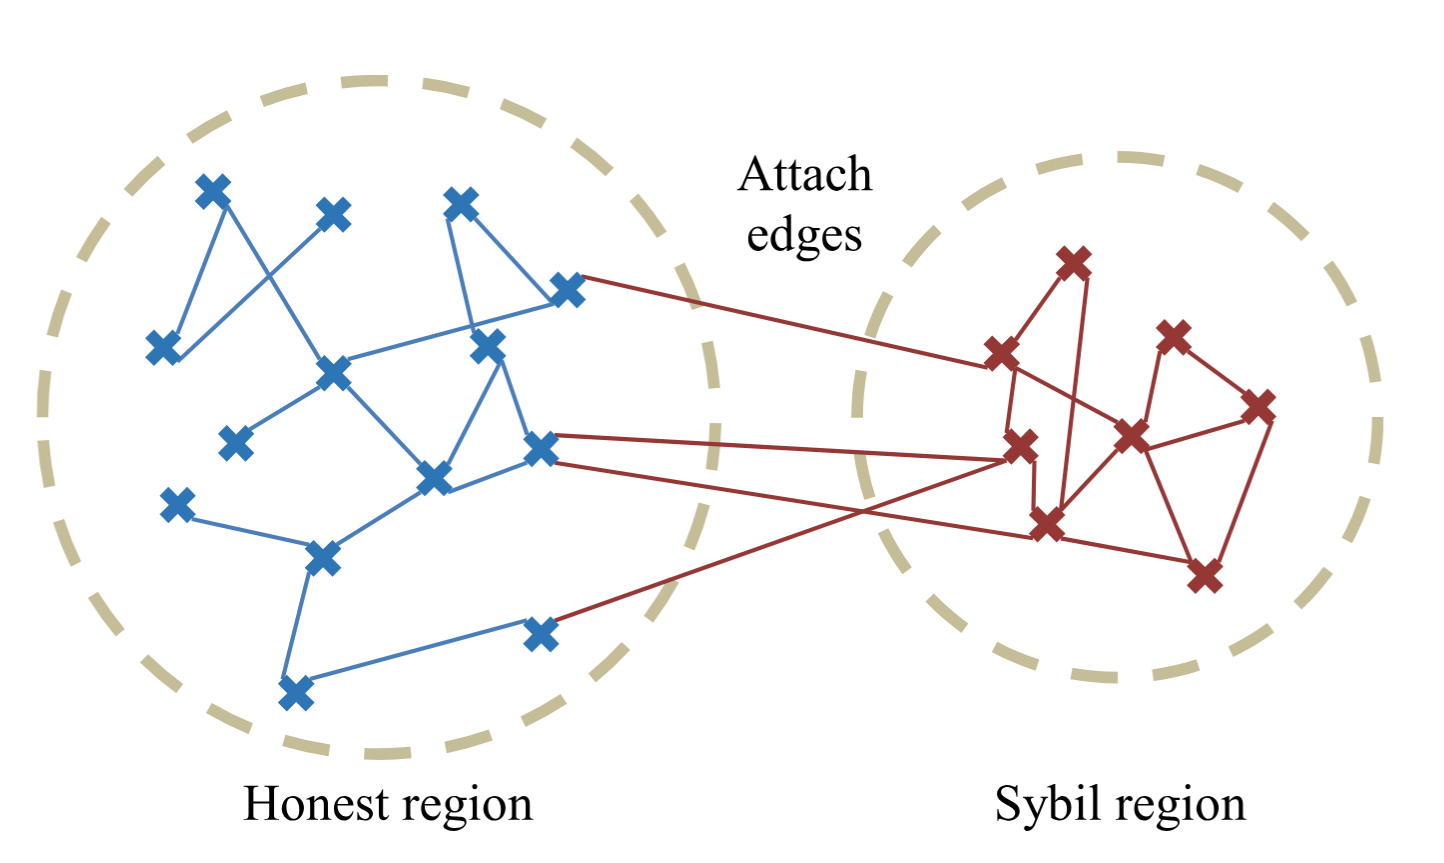
\includegraphics[width=0.6\linewidth]{images/part-02/chap-01/HonestAndSybilRegions.png}
    \vspace{0.2cm}
    \caption{Cấu trúc đồ thị giữa người dùng hợp lệ và mạng lưới Sybil \cite{al2017sybil}}
    \label{fig:HonestSybilRegions}
\end{figure}

Để giải quyết bài toán biểu diễn dữ liệu phức tạp, mạng nơ-ron đồ thị đã trở thành hướng đi chủ đạo. Zhang và cộng sự \cite{zhang2019graph} đã chứng minh hiệu quả của mạng tích chập đồ thị (Graph Convolutional Network, viết tắt là GCN) trong việc học biểu diễn nút, nhưng đồng thời cũng chỉ ra hiện tượng làm mịn quá mức (\textit{over-smoothing}) trên đồ thị siêu đặc. Khắc phục điểm yếu này, Veličković và cộng sự \cite{velickovic2017graph} đề xuất mạng GAT, cho phép mô hình gán trọng số khác nhau cho từng láng giềng. Nhằm tối ưu hóa hơn nữa, Brody và cộng sự \cite{brody2021attentive} đã giới thiệu phiên bản cải tiến GATv2, khắc phục hạn chế của cơ chế chú ý tĩnh ở bản gốc để mang lại khả năng chú ý động vượt trội. Mới đây, Heeb và cộng sự \cite{heeb2024sybil} đã ứng dụng GAT vào phát hiện Sybil, khẳng định ưu thế của cơ chế chú ý trong việc định tuyến tín hiệu dị thường. Bên cạnh đó, nhiều kiến trúc GNN tiên tiến khác cũng đã được đề xuất nhằm nâng cao năng lực biểu diễn cấu trúc, tiêu biểu như mạng đẳng cấu đồ thị tích hợp đặc trưng cạnh (Graph Isomorphism Network with Edges, viết tắt là GINE) \cite{xu2018powerful} với sức mạnh tương đương thuật toán Weisfeiler-Lehman, mạng tổng hợp láng giềng chủ đạo (Principal Neighbourhood Aggregation, viết tắt là PNA) \cite{corso2020principal} sử dụng đa hàm tổng hợp để xử lý các nút có bậc kết nối chênh lệch lớn, hay kiến trúc Graph Transformer \cite{yun2019graph} với khả năng học các phụ thuộc tầm xa trên đồ thị. Song song với việc phát triển cấu trúc truyền tin, việc trích xuất đặc trưng văn bản từ tiểu sử người dùng thông qua các mô hình ngôn ngữ như Sentence-BERT \cite{reimers2019sentence} cũng được kết hợp để làm giàu không gian biểu diễn cho các nút.\vspace{0.3cm}

Mặc dù GNN mang lại hiệu năng cao, thách thức vẫn là sự thiếu hụt dữ liệu nhãn thực tế. Để lấp đầy khoảng trống này, các phương pháp học không giám sát như GAE của Kipf và Welling \cite{kipf2016variational} mở ra tiềm năng trích xuất đặc trưng nhúng mà không cần nhãn. Đồng thời, việc khai thác các đặc trưng cạnh như quyền đồng sở hữu vẫn chưa được các mô hình GNN tiêu chuẩn xử lý tối ưu, dù Gong và Cheng \cite{gong2019exploiting} đã nhấn mạnh tầm quan trọng của chúng.\vspace{0.3cm}

Bên cạnh cấu trúc mạng, phương pháp phân lớp cũng là yếu tố quyết định hiệu năng. Trong các mô hình GNN, các tầng tích chập kết nối trực tiếp với một lớp phân loại tuyến tính. Tuy nhiên, phương pháp này gặp hạn chế do mạng nơ-ron thuần túy thường khó thiết lập các ranh giới phân loại sắc nét, một đặc điểm phân phối cốt lõi của dữ liệu hành vi dạng bảng. Theo Ivanov và Prokhorenkova trong nghiên cứu về \textit{Boosted Graph Neural Networks} \cite{ivanov2021boosted}, mạng nơ-ron thường thiếu chính xác khi đối mặt với các ngưỡng điều kiện nghiêm ngặt. Qua đó, việc sử dụng các mô hình GNN như một bộ trích xuất đặc trưng đang cho thấy nhiều ưu điểm. Phương pháp này kế thừa luận điểm của Grover và Leskovec trong mô hình \textit{node2vec} \cite{grover2016node2vec}, khẳng định khả năng chuyển đổi cấu trúc liên kết và ngữ nghĩa nút thành các vector biểu diễn đặc trưng nút giàu thông tin.\vspace{0.3cm}

Tóm lại, những hạn chế của các nghiên cứu hiện tại nằm ở ba điểm: (1) \textit{Thiếu một quy trình khép kín giải quyết bài toán thiếu nhãn trong môi trường mạng xã hội phi tập trung;} (2) \textit{Chưa tận dụng tối đa các ràng buộc về tính đồng sở hữu đặc thù của Web3;} và (3) \textit{Sự thiếu hụt một kiến trúc đồ thị đa tầng với khả năng tách bạch các tầng quan hệ có nhóm tính chất khác nhau.} Đây chính là động lực để hệ thống \textit{SybilSignal} ra đời, sử dụng đồ thị đa quan hệ nhận thức ràng buộc nhằm tối ưu hóa hiệu năng phát hiện Sybil thông qua việc khai thác chuyên sâu các nhóm quan hệ và đặc trưng phi tuyến.